To have stronger values when we date articles, we wrote a script that runs several times each metrics for a different subset of article of the same year $y$. The idea here is to have an average on the error of each metric to be able to compare them together as follows:
\[
 Mean\_ error = \frac{1}{N} \sum_{i=1}^N \arrowvert p_i - y \arrowvert
\]

where $p_i$ is the prediction at iteration $i$ and $N$ is the number of iterations. We obtained the following results for random years.\\

\textbf{Mean error for different metrics for 15 articles in year 1843 with 15 iterations}\\
\begin{tabular}{p{3cm} p{5cm}}
Distance1 :& 0\\
Cosine :& 10.73333333333333333333\\
Cosine-TFIDF :& .40000000000000000000\\
Chi-Square :& 112.40000000000000000000\\
Kullback-Leibler :& 11.33333333333333333333\\
OutOfPlace :& 3.00000000000000000000\\
Punctuation :& 33.13333333333333333333\\
\end{tabular}\\
 
\textbf{Mean error for different metrics for 15 articles in year 1854 with 15 iterations}\\
\begin{tabular}{p{3cm} p{5cm}}
    Distance1 :& 8.00000000000000000000\\
    Cosine :& 9.86666666666666666666\\
    Cosine-TFIDF :& 0\\
    Chi-Square :& 111.86666666666666666666\\
    Kullback-Leibler :& 0\\
    OutOfPlace :& 8.00000000000000000000\\
    Punctuation :& 15.80000000000000000000\\
\end{tabular}\\
 
\textbf{Mean error for different metrics for 15 articles in year 1888 with 15 iterations}\\
\begin{tabular}{p{3cm} p{5cm}}
    Distance1 :& 42.00000000000000000000\\
    Cosine :& 15.13333333333333333333\\
    Cosine-TFIDF :& 0\\
    Chi-Square :& 62.40000000000000000000\\
    Kullback-Leibler :& .26666666666666666666\\
    OutOfPlace :& 42.00000000000000000000\\
    Punctuation :& 32.80000000000000000000\\
\end{tabular}\\
 
\textbf{Mean error for different metrics for 15 articles in year 1905 with 15 iterations}\\
\begin{tabular}{p{3cm} p{5cm}}
    Distance1 :& 65.80000000000000000000\\
    Cosine :& 17.13333333333333333333\\
    Cosine-TFIDF :& .06666666666666666666\\
    Chi-Square :& 48.40000000000000000000\\
    Kullback-Leibler :& 3.06666666666666666666\\
    OutOfPlace :& 59.00000000000000000000\\
    Punctuation :& 21.06666666666666666666\\
\end{tabular}\\
 
\textbf{Mean error for different metrics for 15 articles in year 1918 with 15 iterations}\\
\begin{tabular}{p{3cm} p{5cm}}
    Distance1 :& 78.93333333333333333333\\
    Cosine :& 4.73333333333333333333\\
    Cosine-TFIDF :& 0\\
    Chi-Square :& 36.33333333333333333333\\
    Kullback-Leibler :& 2.66666666666666666666\\
    OutOfPlace :& 72.00000000000000000000\\
    Punctuation :& 30.86666666666666666666\\
\end{tabular}\\
 
\textbf{Mean error for different metrics for 15 articles in year 1934 with 15 iterations}\\
\begin{tabular}{p{3cm} p{5cm}}
    Distance1 :& 65.60000000000000000000\\
    Cosine :& 17.46666666666666666666\\
    Cosine-TFIDF :& .80000000000000000000\\
    Chi-Square :& 128.93333333333333333333\\
    Kullback-Leibler :& .33333333333333333333\\
    OutOfPlace :& 88.00000000000000000000\\
    Punctuation :& 37.66666666666666666666\\
\end{tabular}\\
 
\textbf{Mean error for different metrics for 15 articles in year 1954 with 15 iterations}\\
\begin{tabular}{p{3cm} p{5cm}}
    Distance1 :& 44.00000000000000000000\\
    Cosine :& 24.60000000000000000000\\
    Cosine-TFIDF :& 0\\
    Chi-Square :& 0\\
    Kullback-Leibler :& .66666666666666666666\\
    OutOfPlace :& 108.00000000000000000000\\
    Punctuation :& 48.06666666666666666666\\
\end{tabular}\\
 
\textbf{Mean error for different metrics for 15 articles in year 1984 with 15 iterations}\\
\begin{tabular}{p{3cm} p{5cm}}
    Distance1 :& 14.00000000000000000000\\
    Cosine :& 7.20000000000000000000\\
    Cosine-TFIDF :& 1.66666666666666666666\\
    Chi-Square :& 3.73333333333333333333\\
    Kullback-Leibler :& 0\\
    OutOfPlace :& 138.00000000000000000000\\
    Punctuation :& 81.80000000000000000000\\
\end{tabular}\\

We observe that two metrics are in general better than the others. These two metrics are the \emph{Kullback-Leibler} Divergence and the Cosine with TF-IDF. Indeed, as explained in section \ref{metrics}, these two metrics are good and we know why. The other metrics are not so bad, even the basic distance which has surprisingly an error of 0 when dating articles from 1843. We think this distance has a good result because the year 1843 is one of the years with the fewer words, so the matching is better than for other years. For the other metrics, we can observe that they vary depending on the year or certainly on the subset of articles.\\

To judge which metric is the best one, we can simply compute the mean error over all our samples. As it takes a lot of time to compute 15 times each metrics, we can't compute it for each year. Here is the overall mean over all the years we tested (1843, 1854, 1888, 1905, 1918, 1934, 1954 and 1984) :\\

\begin{figure}[H]
	\centering
	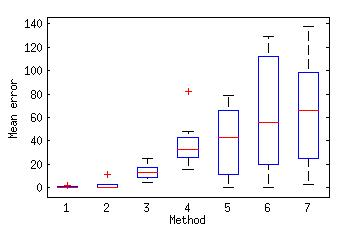
\includegraphics[scale=0.70]{Pictures/date_articles/date_corpus.jpg}
        \caption{Mean error for 15 articles selection and 15 iterations. 1.Cosine TF-IDF, 2.Kullback-Leibler, 3.Cosine, 4.Punctuation, 5.Basic, 6.Chi-Square, 7.Out-of-place}
        \label{date_cv}
\end{figure}

We can observe that, as expected, Cosine with TF-IDF distance and \emph{Kullback-Leibler} Divergence are the best ones.\\

Finally, we made some tests to compare, for a given year, if the number of selected articles to date changes a lot the results of the metrics. We chose to run for a given year (1934) the dating of articles with subsets of articles of sizes 5, 15, 30, 45, 60, 75 and 90. The results are shown in the following table (the smallest distance is colored in green, the biggest in red in table \ref{table_comparison_size_articles}).
\begin{center}
    \begin{table}[h!]
        \begin{tabular}{ | p{3.3cm} | p{1.4cm} | p{1.4cm} | p{1.4cm} | p{1.4cm} | p{1.4cm} | p{1.4cm} | p{1.4cm} | }
            \hline
            \textbf{\# of articles} & \textbf{5} & \textbf{15} & \textbf{30} & \textbf{45} & \textbf{60} & \textbf{75} & \textbf{90}\\
            \hline
            \hline
            \textbf{Basic Distance} & \textcolor{green}{64} & \textcolor{green}{64} & \textcolor{green}{64} & \textcolor{green}{64} & \textcolor{green}{64} & \textcolor{green}{64} & \textcolor{green}{64} \\
            \hline
            \textbf{Cosine} & \textcolor{red}{35} & 18.7334 & 7.7334 & 14.1334 & 6.4667 & \textcolor{green}{4.7334} & 10.7334 \\
            \hline
            \textbf{Cosine-TFIDF} & \textcolor{red}{2.5334} & 0.6667 & 0.1334 & \textcolor{green}{0} & \textcolor{green}{0} & \textcolor{green}{0} & \textcolor{green}{0} \\
            \hline
            \textbf{Chi-Square} & \textcolor{red}{2.1334} & \textcolor{green}{0} & \textcolor{green}{0} & \textcolor{green}{0} & \textcolor{green}{0} & \textcolor{green}{0} & \textcolor{green}{0} \\
            \hline
            \textbf{Kullback-Leibler} & \textcolor{red}{0.0667} & \textcolor{red}{0.0667} & \textcolor{green}{0} & \textcolor{green}{0} & \textcolor{green}{0} & \textcolor{green}{0} & \textcolor{green}{0} \\
            \hline
            \textbf{Out of Place} & \textcolor{red}{89.2} & 88.2667 & \textcolor{green}{88} & \textcolor{green}{88} & \textcolor{green}{88} & \textcolor{green}{88} & \textcolor{green}{88} \\
            \hline
            \textbf{Punctuation} & 46.6 & \textcolor{red}{52.4667} & 38.0667 & 29.6667 & 38.4667 & \textcolor{green}{29.0667} & 32.8667 \\
            \hline
        \end{tabular}
        \caption{Mean error distance for the year 1934 with different numbers of articles for 15 iterations}
        \label{table_comparison_size_articles}
    \end{table}
\end{center}

We observe that in general, more we have articles, better is the dating. First, we have to note that more we take articles, more we remove words in the article's year which can make the number of words in this year consequently smaller than other years. It could be an explanation why taking a lot of articles to date them is not necessarily a good thing (for cosine distance for example). Nevertheless, we observe that the punctuation distance prefers a bigger set of articles, because it can have a better approximation of the sentences length, number of commas and so on for the article's year. It is also the case for all the metrics. Indeed, for \emph{Kullback-Leibler}, Cosine, Cosine with TF-IDF and Out of Place distance, once the minimum distance is obtained, it seems that it does not change. We can explain this phenomenon by the fact that adding more information for dating is useless once we have reached the minimum possible distance. For the basic distance, the gap of 64 years is probably because the predicted year is 1998. This distance predict 1998 because in this year the number of words is much smaller than in other years (the data cover not all the year because of a merging of newspaper). Due the size of 1998, the basic distance should always have a better connection with it.